\documentclass[12pt]{article}
\usepackage{bm}
\usepackage{graphicx}
\usepackage{gensymb}
\usepackage{float}
\usepackage{siunitx}
\usepackage{listings}
\usepackage{hyperref}
\usepackage[a4paper, total={6in, 8in}]{geometry}

\graphicspath{{./../images/}}

\begin{titlepage}

\title{\textbf{Optimum Loft Angle for Greatest Carry Distance}}
\author{\textbf{Group D}\\
		Alison McIntosh\\
		Emily Dark\\
		Henry Archer\\
		Kyle Stewart\\
		Stuart Ballantyne}
\date{}

\end{titlepage}

\begin{document}

\begin{titlepage}
\maketitle
\thispagestyle{empty}
\pagebreak
\end{titlepage}

\pagenumbering{arabic}

\section{Response}
The loft angle of the golf club which maximises the range of the golf ball trajectory is referred to as the optimum loft angle. This investigation consisted of two main parts: the impact of the club, and the flight of the golf ball. The golf ball considered is the Titleist Pro V1x, with characteristics outlined under (2.1) Assumptions.

\subsubsection{Atmospheric conditions at different golf courses}
\begin{table}[H]
\caption{Atmospheric conditions at each golf course}
\label{tab:aconditions}
\resizebox{\textwidth}{!}{%
\begin{tabular}{|l|l|l|l|l|}
\hline
Location                  & Temperature ($K$) & Humidity ($\%$) & Altitude ($m$) & Air density ($kg/m^3$)		\\ \hline
Renaissance, East Lothian &  287            & 85            & 84         & 1.128                              \\ \hline
La Paz, Bolivia           & 278             &60             & 3342         & 0.861                               \\ \hline
Sentosa, Singapore        & 307              &  75        & 33      & 1.154                               \\ \hline
\end{tabular}%
}
\end{table}

The tournament in Singapore took place in January 17th-20th 2019.The tournament in East Lothian is scheduled to take place in July, 8th-14th (2019) and the Bolivian tournament is scheduled for August (2019). The values for temperature and humidity are average values for the given time of year.

\subsection{Results}
The following graphs are for the conditions at Renasissance, East Lothian.

\begin{figure}[H]
\centering
\caption{Effect of loft angle on carry distance}
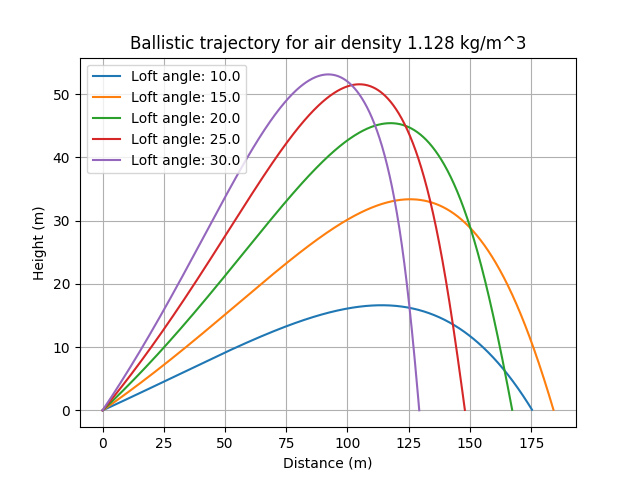
\includegraphics[scale=0.6]{results1128}
\end{figure}

\begin{figure}[H]
\centering
\caption{Loft angle vs carry distance to obtain optimum loft angle}
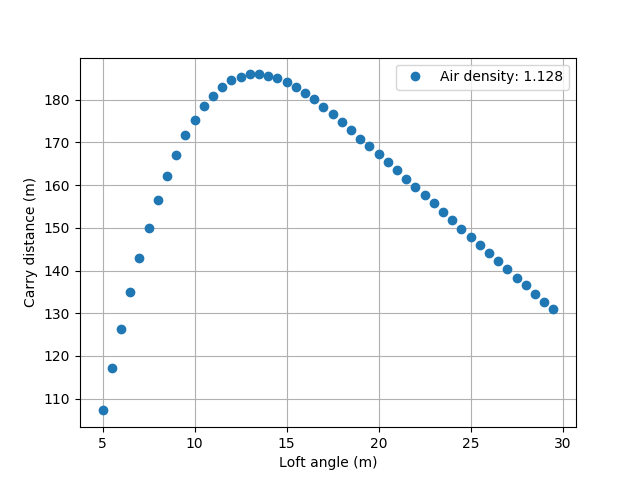
\includegraphics[scale=0.6]{results1128range}
\end{figure}

From the investigation, the recommended loft angle to maximise the carry distance based on a club speed of 51.4 $ms^-1$  for the Scottish Open at the Renaissance Club in East Lothian is \SI{13.4}{\degree} which produces a flight distance of \SI{186}{\metre}.

The following graphs are for the conditions at La Paz, Bolivia.

\begin{figure}[H]
\centering
\caption{Effect of loft angle on carry distance}
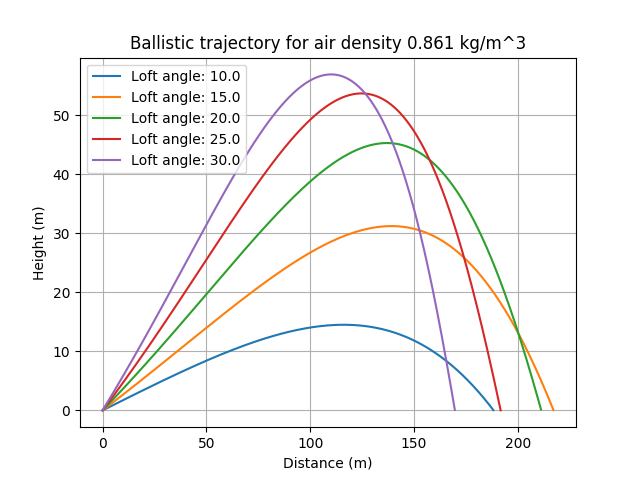
\includegraphics[scale=0.6]{results0861}
\end{figure}

\begin{figure}[H]
\centering
\caption{Loft angle vs carry distance to obtain optimum loft angle}
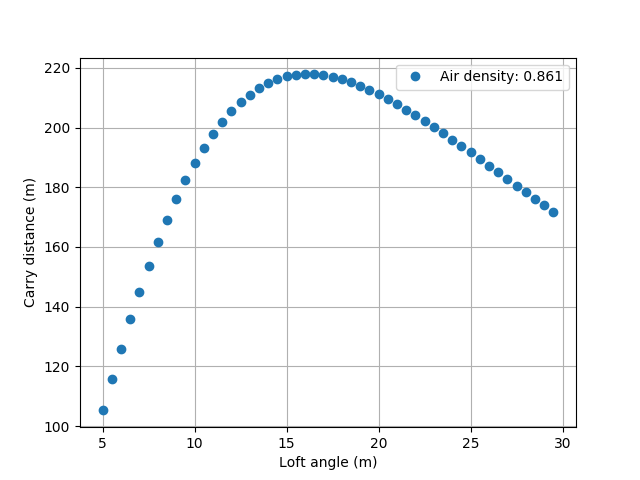
\includegraphics[scale=0.6]{results0861range}
\end{figure}

The recommended loft angle to maximise the flight distance based on a club speed of \SI{51.4}{\metre\per\second} for the La Paz golf club in Bolivia is \SI{16.2}{\degree} which produces a carry distance of \SI{218}{\metre}.
 
 The following graphs are for the conditions at Sentosa, Singapore.

\begin{figure}[H]
\centering
\caption{Effect of loft angle on carry distance}
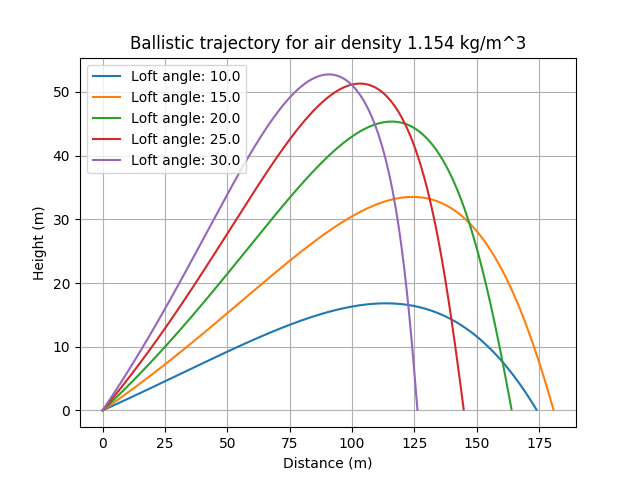
\includegraphics[scale=0.6]{results1154}
\end{figure}

\begin{figure}[H]
\centering
\caption{Loft angle vs carry distance to obtain optimum loft angle}
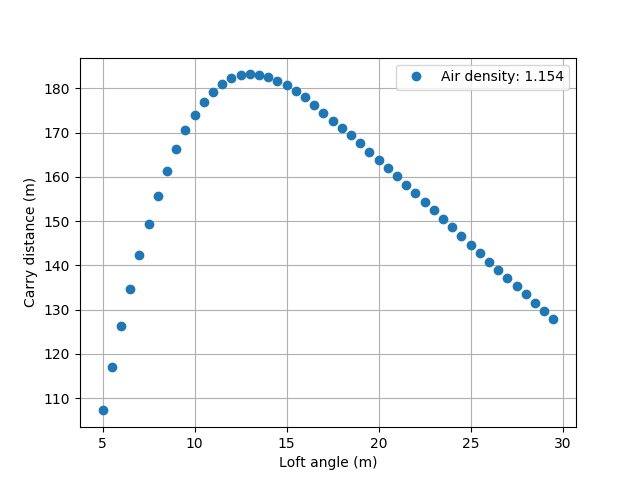
\includegraphics[scale=0.6]{results1154range}
\end{figure}

The recommended loft angle to maximise the flight distance based on a club speed of \SI{51.4}{\metre\per\second} for the Sentosa, is \SI{13.2}{\degree} which produces a carry distance of \SI{183}{\metre}.
 






\begin{figure}[H]
\centering
\caption{Effect of club speed on carry distance and optimum loft angle, $\omega_{spin}=$ \SI{300}{\radian\per\second}, $v_i =$ \SI{50}{\metre\per\second}}
\includegraphics[scale=0.6]{effectofairdensity2}
\end{figure}








\section{Theory}

\subsection{Assumptions}
The following assumptions are made throughout the report and model:
\begin{description}
  \item[$\cdot$] golf course is level and has no effect on trajectory;
  \item[$\cdot$] height of the tee is negligible;
  \item[$\cdot$] gravitational field strength is constant (\SI{9.81}{\metre\per\second^{2}}) and does not flucuate with height;
  \item[$\cdot$] driver is roughly a flat plate and strikes the ball precisely at the center, with no draw or fade;
  \item[$\cdot$] the mass of the club head is significantly greater than that of the shaft, so we consider the shaft's influence to be neglible;
  \item[$\cdot$] the golf ball is a Titleist Pro V1x, with a mass of \SI{45.93}{\gram}, diameter of \SI{42.67}{\milli\metre}, a moment of inertia of \SI{0.009145}{\gram\cdot\metre^2}, and 352 circular dimples.
\end{description}

\subsection{Impact}
\subsubsection{Conservation of energy}
The collision between the club head and golf ball is inelastic, meaning the kinetic energy of the system is not conserved, but rather some of the energy is converted into different forms. One such form is elastic energy in the deformation of the golf ball. This has significant effect on the initial velocity of the golf ball, as the more the ball is deformed, the less kinetic energy the ball will have after the collision. The coefficient of restitution $e$ is the ratio of the final and initial velocities between the golf ball and club head after the collision and it is introduced in calculations. Further energy is lost as heat and sound.

\subsubsection{Conservation of momentum}
The law of conservation of momentum was applied and the velocities were resolved into components.
\begin{equation} \label{linearmomentum1}
M v_{cfn}+mv_{bfn}=Mv_{ci} \cos{\theta}
\end{equation}
\begin{equation} \label{linearmomentum2}
M v_{cfp}+mv_{bfp}=-Mv_{ci} \sin{\theta}
\end{equation}
$v_{bfn}$ and $v_{bfb}$ can be expressed in terms of $v_{ci}$, the initial club speed, as equations (\ref{clubspeed1}-\ref{clubspeed2}).

\begin{equation} \label{clubspeed1}
v_{bfn}=(1+e)v_{ci} \frac{\cos{\theta}}{1+\frac{m}{M}}
\end{equation}
\begin{equation} \label{clubspeed2}
v_{bfp}=-v_{ci} \frac{\sin{\theta}}{1+\frac{m}{M}+\frac{mr^2}{I}}
\end{equation}
These two vector components can be added to yield $v_{bo}$ and $\phi_{bo}$, the velocity and its direction for the ball on departure; equations (\ref{initialvelocity}-\ref{launchanglephi})\cite{Penner2001}
\begin{equation} \label{initialvelocity}
v_{bo}=v_{bf}=\sqrt{v_{bfn}^2+v_{bfp}^2}
\end{equation}
\begin{equation} \label{launchanglephi}
\phi_{bo}=\theta+\tan^{-1}{\frac{v_{bfp}}{v_{bfn}}}
\end{equation}

Lieberman and Johnson give values for $e$ decreasing from approximately $0.76$ for impact speeds of \SI{37}{\metre\per\second} to values of around $0.72$ for impact speeds of \SI{50}{\metre\per\second}. Applying a linear fit gives the empirical equation (\ref{restitution})\cite{Penner2001}.
\begin{equation} \label{restitution}
e=0.86-0.0029 v_{impact} \cos{\theta}
\end{equation}


\begin{figure}[H]
\centering
\caption{Loft angle and spin}
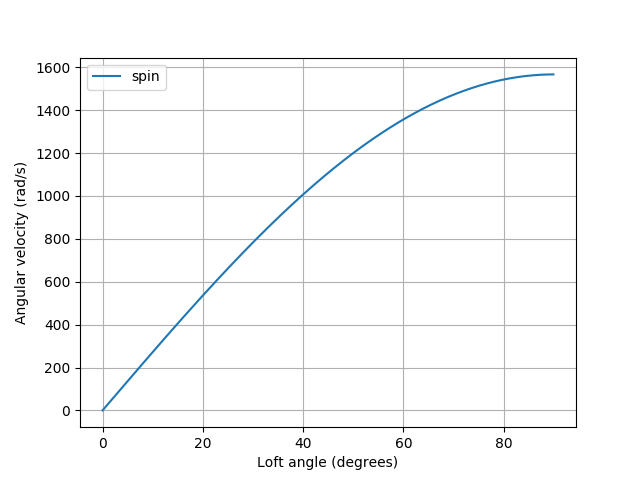
\includegraphics[scale=0.6]{loftangleandspin}
\end{figure}


\subsection{Flight conditions}
The main atmospheric factor affecting the golf ball’s flight is air density which is dependent on air pressure, temperature and humidity. When air density increases, there is increased resistance against the ball during its flight, thus the maximum carry distance is less. Air molecules have greater kinetic energy as the temperature of the air increases, causing them to occupy a larger volume. This results in a decrease in air density. When the air pressure is increased, air density also increases as more collisions between particles occur. The relative humidity of air is a measure of the water vapour relative to temperature and is the percentage of water vapour that could potentially be held in the air at that given temperature.  The air density of humid air is less than dry air. Relative humidity is given by equation (\ref{pressures}):
\begin{equation} \label{pressures}
\phi = \frac{P_w}{P_{w}^\prime} \times 100
\end{equation}
where $P_w$ is the pressure for water vapour and $P_{w}^\prime$ is the equilibrium vapour pressure, that is the maximum pressure it could be in that given temperature value. This value of $P_{w}^\prime$ can be obtained by Antoine's equation (\ref{antoine}) \cite{Roizard2014}:
\begin{equation} \label{antoine}
P_{w}^\prime = e^{\frac{A-B}{C+T}}
\end{equation}
where $T$ is the temperature in K and $A$, $B$, and $C$ are are component specific constants for the given medium. Through the use of Dalton's law for partial pressures, the molar fraction of elements which compose the atmosphere can be calculated using equation (\ref{daltons}):
\begin{equation} \label{daltons}
x_w = \frac{P_w}{P_T}
\end{equation}
where $x_w$ is the molar fraction of water vapour and $n_T$ is the total number of moles which is obtained using the ideal gas law (\ref{idealgaslaw}):
\begin{equation} \label{idealgaslaw}
P_T V = n_T R T
\end{equation}
where $P_T$ is the total pressure, which is found using the barometric formula (\ref{barometric}) \cite{BerberanSantos1997}:
\begin{equation} \label{barometric}
P_T = P_0 e^{\frac{-Mg}{R T_0} h}
\end{equation}
where $P_0$ and $T_0$ are, respectively, pressure and temperature at sea level (\SI{103125}{\pascal}, \SI{288.15}{\kelvin}), $g$ is the gravitational field strength, L is the temperature lapse rate (\SI{0.0065}{\kelvin\per\metre}). At higher altitudes, the air molecules can spread out further resulting in a decrease in air density.\\
The molar fraction of water vapour can be obtained through equation (\ref{molar})
\begin{equation} \label{molar}
x_w = \frac{n_w}{n_T}
\end{equation}
From here, the number of moles for each major component of the atmosphere - nitrogen, oxygen, argon, and water vapour - was obtained using equation (\ref{components}):
\begin{equation} \label{components}
n_T - n_w = n_O + n_N + n_{Ar}
\end{equation}
and considering the fraction of each component of air:
\begin{equation}
n_N = 0.7808(n_T - n_w)
\end{equation}
\begin{equation}
n_O = 0.20195(n_T - n_w)
\end{equation}
\begin{equation}
n_{Ar} = 0.0093(n_T - n_w)
\end{equation}
By the consideration of the molar masses, the density of air can be calculated by the equation (\ref{airdensity}):
\begin{equation} \label{airdensity}
\rho = \frac{((M_N P_{N}) + (M_O P_{O}) + (M_{Ar} P_{Ar}))}{RT}
\end{equation}
where $P$ is the partial pressure of an element, found by equation (\ref{ppressures}):
\begin{equation} \label{ppressures}
P = \frac{n_x RT}{V}
\end{equation}
where $n_x$ is the number of moles for a given element. Consequently, this allowed the air density to be found for each course based on environmental conditions. \cite{Legg2017}

\subsection{Flight}
\subsubsection{Simple golf ball}
A simple golf ball experiencing only weight may be modelled by the following system of differential equations;
\begin{equation} \label{simpleaccelx}
a_x=\frac{\partial v_x}{\partial t}=0
\end{equation}
\begin{equation} \label{simpleaccely}
a_y=\frac{\partial v_y}{\partial t}=-g
\end{equation}
where $g$ is the gravitional field strength.

Assuming the initial velocity is $v_0$ and the launch angle is $\theta$, equations (\ref{simpleaccelx}-\ref{simpleaccely}) can be solved to give equations (\ref{simplevelx}-\ref{simplevely}):
\begin{equation} \label{simplevelx}
v_x=v_0 \cos{\theta}
\end{equation}
\begin{equation} \label{simplevely}
v_y=v_0 \sin{\theta}-gt
\end{equation}
Integrating equations (\ref{simplevelx}-\ref{simplevely}) with respect to time yields the displacement as a function of time to give equations (\ref{simpleposx}-\ref{simpleposy}) \cite{Penner2001}:
\begin{equation} \label{simpleposx}
x=v_0 t \cos{\theta}
\end{equation}
\begin{equation} \label{simpleposy}
y=v_0 t \sin{\theta}-\frac{1}{2} g t^2
\end{equation}

\begin{figure}[H]
\centering
\caption{Golf ball trajectory, no drag or lift}
\includegraphics[scale=0.6]{simple}
\end{figure}

\begin{figure}[H]
\centering
\caption{Range as a function of loft angle, no drag or lift}
\includegraphics[scale=0.6]{simplerange}
\end{figure}

Figures (1-2) show the maximum range is when the loft angle at 45.0\degree, as predicted by the equations of projectile motion.
\subsubsection{Smooth golf ball experiencing drag}
The drag equation (\ref{drageqn})
\begin{equation} \label{drageqn}
\vec{F_{d}} = \frac{1}{2} A C_{d} \rho_{air} |\vec{v}| \vec{v}
\end{equation}
where $\rho_{air}$ is the density of air; $A$ is the reference area, which in the case of a smooth sphere of radius $r$, is the cross-sectional area $\pi r^2$; $C_d$ is the coefficient of drag, which is dependent on the Reynolds number; and $\vec{v}$ is the flow velocity relative to the golf ball. In this case, we assume the air is stationary and the golf ball is moving through the air with velocity $\vec{v}$.

Applying equation (\ref{drageqn}) to equations (\ref{simpleaccelx}-\ref{simpleaccely}), we get
\begin{equation} \label{dragaccelx}
\frac{\partial v_x}{\partial t}=-k |v_x| v_x
\end{equation}
\begin{equation} \label{dragaccely}
\frac{\partial v_y}{\partial t}=-g-k |v_y| v_y
\end{equation}
where $k=\frac{1}{2} A C_d \rho_{air}$. These equations already do not have a closed-form solution and require numerical methods.
\begin{figure}[H]
\centering
\caption{Golf ball trajectory when experiencing drag but no lift, $C_d$ = 0.5}
\includegraphics[scale=0.6]{dragcd}
\end{figure}

\begin{figure}[H]
\centering
\caption{Range as a function of loft angle, $C_d$ = 0.5}
\includegraphics[scale=0.6]{dragcdrange}
\end{figure}

Figure (4) shows that the maximum range is achieved at 40.2\degree, for an initial velocity of \SI{50}{\metre\per\second}. Additionally, the range is significantly decreased when drag was added to the model. The greatest range with drag is about \SI{114}{\metre} versus the previous range of \SI{255}{\metre} at 45.0\degree.
However, $C_d$ is not constant and depends on the Reynolds number, which is proportional to the velocity of the golf ball. The Reynolds number is given by equation (\ref{reynolds})\cite{Alam2011}:
\begin{equation} \label{reynolds}
R=\frac{2vr}{\nu}
\end{equation}
where $\nu$ is the kinematic viscosity of air.

Using data from \textit{Alam 2011}\cite{Alam2011}, Python was used to construct a quartic fit of drag coeffiecient as a function of Reynolds Number, as shown in Figure (5).\\
A quartic approximation is best as any greater degree would begin to oscillate too much at the edges (Runge's phenomenon). Likewise, a lesser degree would be too linear to give any meaningful relation.\\
One of the limitions of this approach is that there is no data above Reynolds number $112,000$ (\SI{38.39}{\meter\per\second}) or below $63,300$ (\SI{21.70}{\meter\per\second}), so the approximation does not hold for those conditions, and may in fact be drastically worse due to the chaotic behaviour of the polynomial at the aforementioned values. To overcome this, the drag coefficient was fixed at 0.8 for Reynolds numbers less than 53,000 and fixed at 0.37 for Reynolds numbers greater than 120,000.


\begin{figure}[H]
\centering
\caption{Drag coefficient as a function of Reynolds number with curve of best fit}
\includegraphics[scale=0.6]{reynolds}
\end{figure}

Applying the approxmation for the coefficient of drag, the optimum loft angle decreases down to about 34.5\degree, shown in figures (6-7).
\begin{figure}[H]
\centering
\caption{Trajectory of golf ball with drag considering Reynolds number, $v_i=$ \SI{50}{\metre\per\second}}
\includegraphics[scale=0.6]{dragwithreynolds}
\end{figure}

\begin{figure}[H]
\centering
\caption{Range against loft angle for golf ball with drag considering Reynolds number, $v_i=$ \SI{50}{\metre\per\second}}
\includegraphics[scale=0.6]{dragwithreynoldsrange}
\end{figure}


\subsubsection{Smooth golf ball experiencing lift}
Lift on a golf ball is caused by the Magnus effect, which is dependent on the backspin of the ball. The equation is similar to the drag equation, however the direction of the force is perpendicular to both angular velocity and translational velocity.

\begin{equation} \label{lifteqn}
F_l = \frac{1}{2} \rho_{air} C_{l} |v|^2 (\hat{\omega} \times \hat{v})
\end{equation}

where $C_l$ is dependent on the spin parameter of the ball according to \cite{Bearman1976}.
\begin{equation} \label{clifteqn}
C_l = -3.25 S^2 + 1.99 S
\end{equation}
The spin parameter is given by the ratio of the magnitude of tangential velocity to the magnitude of translational velocity.
\begin{equation} \label{spineqn}
S = \frac{r|\omega|}{|v|}
\end{equation}


\bibliography{bibliography}{}
\bibliographystyle{plain}

\pagebreak

\lstdefinestyle{PythonStyle}{
  language=Python,
  numbers=left,
  stepnumber=1,
  numbersep=10pt,
  tabsize=4,
  showspaces=false,
  showstringspaces=false
}

\textit{The model was written using Python version 3.8, on a Linux machine, although earlier versions (i.e. 3.5) should work. It requires the following Python packages: NumPy, SciPy, and Matplotlib. Use ./model3d.py -h for a list of parameters. It also supports 3d plots, though these are experimental. The source code is also hosted as a git repository at \url{https://github.com/s-ballantyne/gdp}.}
\begin{lstlisting}[language=Python, caption=Python model), style=PythonStyle, basicstyle=\tiny]
#!/usr/bin/env python3

import numpy as np
import argparse

from scipy.integrate import odeint as integrate
from matplotlib import pyplot as plot
from numpy.linalg import norm
from mpl_toolkits.mplot3d import Axes3D

parser = argparse.ArgumentParser()

# Ball parameters
constants = parser.add_argument_group("Constants")
constants.add_argument("-m", "--mass", default=0.04593, help="Mass of ball (kg)")
constants.add_argument("-r", "--radius", default=0.04267/2, help="Radius of ball (m)")

constants.add_argument("-g", "--gravity", type=float, default=9.81, help="For when we get a Mars base (m/s/s)")
constants.add_argument("-d", "--density", type=float, default=1.225, help="Density of air (kg m^-3)")
constants.add_argument("--viscosity", type=float, default=1.46e-5, help="Kinematic viscosity of air")

# Initial parameters
initialparams = parser.add_argument_group("Initial parameters")
#initialparams.add_argument("-vi", "--velocity", type=float, default=50, help="Initial velocity (m/s)")
initialparams.add_argument("-yi", "--height", type=float, default=0, help="Initial height (m)")

#initialparams.add_argument("-sp", "--spin", type=float, default=0, help="Spin (z)")
#initialparams.add_argument("-spy", "--spiny", type=float, default=0, help="Spin (y)")
#initialparams.add_argument("-spx", "--spinx", type=float, default=0, help="Spin (x)")

# Loft angle
parser.add_argument("-li", "--loftinitial", type=float, default=10, help="Loft angle (initial)")
parser.add_argument("-lf", "--loftfinal", type=float, default=35, help="Loft angle (final)")
parser.add_argument("-st", "--step", type=float, default=5, help="Loft angle (step)")

# Debugging
parser.add_argument("-v", "--verbose", action="store_true")

# Ball speed calculations
parser.add_argument("--clubmass", type=float, default=0.2, help="Mass of club head (kg)")
parser.add_argument("--vclub", type=float, default=51.4, help="Club speed (m/s)")
parser.add_argument("--inertia", type=float, default=9.145e-6, help="Inertia of golf ball")

# Parse args
args = parser.parse_args()

# Input validation
assert args.loftfinal > args.loftinitial, "Final loft angle must be gretaer than initial loft angle!"
assert args.step != 0, "Step must be non-zero!"
assert ((args.loftfinal - args.loftinitial) / args.step).is_integer(), "Step size must divide the change in loft angle!"

assert args.mass != 0, "Mass must be non-zero."
assert args.radius != 0, "Radius must be non-zero."
assert args.viscosity != 0, "Kinematic viscosity must be non-zero."
assert args.density != 0, "Density of air must be non-zero."

g = args.gravity
density = args.density

# Ball speed from club speed and loft angle
def ball_speed(theta):
	theta = np.radians(theta)
	e = 0.86 - 0.0029 * args.vclub * np.cos(theta)

	bfn = (1 + e) * args.vclub * np.cos(theta) / (1 + args.mass / args.clubmass)
	bfp = args.vclub * np.sin(theta) / (1 + args.mass / args.clubmass + (args.mass * args.radius**2 / args.inertia))
	return np.sqrt(bfn**2 + bfp**2)

# Spin
def ball_spin(theta):
	theta = np.radians(theta)
	bfp = args.vclub * np.sin(theta) / (1 + args.mass / args.clubmass + (args.mass * args.radius**2 / args.inertia))

	return args.mass * bfp * args.radius / args.inertia

# Coefficient of drag from Reynolds number, based on degree four polynomial.
def re_to_cd(re):
	# Clamp output value as it is only an approximation
	if re > 120000:
		return 0.370
	elif re < 53000:
		return 0.8

	# Array of coefficients
	coeffs = np.array([
			  9.46410458e-20, -3.80736984e-14,
			  5.72048806e-09, -3.81337408e-04,
			  9.92620188e+00
			])

	# Return value of polynomial approximation
	return np.polyval(coeffs, re)


# Linear velocity to Reynolds number (Re = velocity * diameter / k. viscosity)
def reynolds(velocity, radius):
	return 2 * radius * velocity / args.viscosity


# Linear velocity to drag coefficient
def sphere_cd(velocity, radius):
	cd = re_to_cd(reynolds(velocity, radius))
	return cd


# Drag equation
# F_d = 1/2 * air density * ref. area * coefficient * |velocity| * v
def drag(density, area, cd, velocity):
	return -0.5 * density * area * cd * norm(velocity) * velocity


# Lift equation
# F_l = 1/2 * air density * ref. area * coefficient * |v|^2 * (what x vhat)
def lift(density, area, cl, velocity, rvelocity):
	if cl == 0:
		return np.array([0, 0, 0])

	S = 0.5 * density * area * cl

	# Cross product of angular velocity and linear velocity, for direction of spin
	rxv = np.cross(rvelocity, velocity)
	rxv /= norm(rxv)

	# Magnitude of spin is considered in coefficient of lift
	return S * norm(velocity)**2 * rxv

# Simple golfball, no drag, no lift, smooth
class BasicGolfball:
	def __init__(self):
		# Properties
		self.mass = args.mass
		self.radius = args.radius

		# Coordinates
		self.x = 0
		self.y = args.height
		self.z = 0

		self.vx = 0
		self.vy = 0
		self.vz = 0

		# Rotational velocities
		self.rvx = 0
		self.rvy = 0
		self.rvz = 0

	# Reference area, for a sphere this is the cross-section.
	def area(self):
		return np.pi * self.radius**2

	# Set initial velocity
	def set_velocity(self, v, theta):
		self.vx = v * np.cos(np.radians(theta))
		self.vy = v * np.sin(np.radians(theta))

	# Set spin
	def set_spin(self, spin):
		self.rvx, self.rvy, self.rvz = spin

	# Get all coordinates
	def coords(self):
		return np.array([self.x, self.y, self.z, self.vx, self.vy, self.vz, self.rvx, self.rvy, self.rvz])

	# Set all coordinates [x, y, z, vx, vy, vz, rvx, rvy, rvz]
	def set_coords(self, coords):
		self.x, self.y, self.z, self.vx, self.vy, self.vz, self.rvx, self.rvy, self.rvz = coords

	# Returns numpy array of position coordinates
	def position(self):
		return np.array([self.x, self.y, self.z])

	# Returns numpy array of velocity at the current position
	def velocity(self):
		return np.array([self.vx, self.vy, self.vz])

	# Returns numpy array of acceleration at the current position
	def acceleration(self):
		return np.array([0, -g, 0])

	# Returns numpy array of rotational velocity (spin) at the current position
	def rvelocity(self):
		return np.array([self.rvx, self.rvy, self.rvz])

	# Returns numpy array of rotational acceleration at the current position
	def racceleration(self):
		return np.array([0, 0, 0])

	# Returns numpy array of differential eqns to be solved by odeint
	def differentials(self):
		d = np.zeros(9)

		d[0:3] = self.velocity()
		d[3:6] = self.acceleration()

		d[6:9] = self.racceleration()

		return d

	# (Internal) Updates coordinates and returns list of equations to solve (for odeint)
	def __eqns(self, t, coords):
		self.set_coords(coords)

		if args.verbose:
			print(t, self.velocity(), self.rvelocity(), self.acceleration(), self.racceleration())

		return self.differentials()

	# Solve for trajectory over given interval
	def solve(self, t0, t1, dt=0.01):
		interval = np.linspace(t0, t1, int((t1 - t0) / dt))
		res = integrate(self.__eqns, self.coords(), interval, tfirst=True)[:, :3]

		out = np.array([e for e in res if e[1] >= 0])
		return out

# Simple golf ball but with drag
class DragGolfball(BasicGolfball):
	def __init__(self):
		BasicGolfball.__init__(self)

	# Coefficient of drag from velocity & radius
	def cd(self):
		return sphere_cd(norm(self.velocity()), self.radius)

	def acceleration(self):
		fd = drag(density, self.area(), self.cd(), self.velocity())
		return BasicGolfball.acceleration(self) + fd / self.mass


# Golfball with lift and drag
class LiftGolfball(DragGolfball):
	def __init__(self):
		DragGolfball.__init__(self)

	# Returns spin factor
	def spinf(self):
		v = norm(self.velocity())
		w = self.radius * norm(self.rvelocity())
		return w / v

	# Returns coefficient of lift based on spin factor
	def cl(self):
		s = self.spinf()
		return -3.25 * s**2 + 1.99 * s

	def acceleration(self):
		fl = lift(density, self.area(), self.cl(), self.velocity(), self.rvelocity())
		return DragGolfball.acceleration(self) + fl / self.mass

	# Spin decreases by about 1% every second
	def racceleration(self):
		return -0.01 * self.rvelocity()


if __name__ == "__main__":
	# Initial conditions
	for density in [1.128, 0.861, 1.154]:
		plot.figure()
		for theta in np.arange(args.loftinitial, args.loftfinal, args.step):
			ball = LiftGolfball()
			ball.set_velocity(ball_speed(theta), theta)
			ball.set_spin([0, 0, ball_spin(theta)])

			res = ball.solve(0, 10)
			x, y, z = res.T

			plot.plot(x, y, label="Loft angle: " + format(theta, ".1f"))

		plot.legend()
		plot.grid(True)
		plot.xlabel("Distance (m)")
		plot.ylabel("Height (m)")
		plot.title("Ballistic trajectory for air density " + format(density, ".3f") + " kg/m^3")

		plot.figure()
		xdata = []
		ydata = []
		for theta in np.arange(5, 30, 0.5):
			ball = LiftGolfball()
			ball.set_velocity(ball_speed(theta), theta)
			ball.set_spin([0, 0, ball_spin(theta)])

			res = ball.solve(0, 10)
			x, y, z = res.T

			xdata.append(theta)
			ydata.append(x[-1])

		plot.plot(xdata, ydata, 'o', label="Air density: " + format(density, ".3f"))
		plot.legend()
		plot.grid(True)
		plot.xlabel("Loft angle (m)")
		plot.ylabel("Carry distance (m)")

	plot.show()
\end{lstlisting}


\end{document}


\grid
